\documentclass[11pt]{article}
\usepackage[margin=1.1in]{geometry}
\usepackage{amsmath,amssymb}
\usepackage{booktabs}
\usepackage{graphicx}
\usepackage[hidelinks]{hyperref}
\usepackage{xcolor}
\usepackage{pgfplots}
\pgfplotsset{compat=1.17}
\definecolor{accent}{RGB}{42,101,175}
\definecolor{corrupt}{RGB}{201,109,44}
\definecolor{inkmut}{RGB}{110,118,126}

\title{Instructions Buy the Phrase; the Phrase Costs Preference:\\
an Epistemic Audit of LLM Aggregation Pipelines at Auditable Scale}
\author{Sam Bobo\\ \small with analysis assistance from Claude (Anthropic)}
\date{Draft v0.1 --- August 2026}

\newcommand{\ci}[2]{\ensuremath{[#1,\,#2]}}

\begin{document}
\maketitle

\begin{abstract}
Mixture-of-Agents (MoA) pipelines --- proposer models whose outputs an
aggregator synthesizes --- achieve state-of-the-art results on
preference-judged benchmarks, but every published gain is measured by an
LLM preference judge, and nothing in that literature measures what such
gains are made of. We audit the MoA architecture at auditable scale
(7--20B local models) with pre-registered cells, validated instruments,
and causal designs, and report three linked findings. (1)~A
phrase-swap experiment shows that an epistemic instruction (``label
estimates with phrase $X$'') produces \emph{only} its named phrase: the
dictated form appears in two thirds of outputs regardless of which
synonym is named, while the construct rate outside the named phrase is
statistically unchanged (CIs $\ci{-0.079}{+0.111}$,
$\ci{-0.103}{+0.087}$). (2)~A preference judge, order-debiased, shows a
real aggregation lift --- the aggregated pipeline beats the same writer
answering directly in $0.818$ \ci{0.718}{0.919} of decisive pairs,
surviving length matching --- yet \emph{penalizes} the instructed arms:
the phrase-bearing arms lose to their own control in both
counterbalanced forms ($0.261$ \ci{0.140}{0.388}; $0.317$
\ci{0.152}{0.480}). Because the arms differ only in the phrase, the
penalty is causally attributable to it. Together these results identify
a measured tension: instruction tuning of epistemic disposition installs
surface forms, and preference optimization removes exactly those forms.
(3)~The preference instrument itself is majority reading-order at this
scale: raw first-position preference is $0.85$, order-debiasing converts
two thirds of pairs to ties, and a second local judge produced $95\%$
ties. We further report mechanism results that bound the MoA narrative
--- the aggregator selects sources rather than recomputing, ignores
cross-proposer corroboration, and transports roughly $15\%$ of upstream
epistemic qualification --- and release the measurement kit, the
dictation registry, and all pre-registrations.
\end{abstract}

\section{Introduction}

Mixture-of-Agents \cite{wang2024moa} reports that a stack of open-source
proposers plus an aggregator surpasses GPT-4o on AlpacaEval~2.0 (65.1\%
vs.\ 57.5\% length-controlled win rate), and frames the result as
``collaborativeness'': models produce better responses when shown other
models' outputs, even lower-quality ones. Every number in that paper ---
and in the surrounding multi-agent literature --- is produced by an LLM
preference judge. No published MoA evaluation measures a verifiable
outcome, tests error propagation, validates its judge on the deployed
task, or separates behavioral change from surface compliance.

This paper supplies that audit. It is the product of a
falsification-first research program that ran forty-three pre-registered
experiment cells on a MoA-architecture pipeline small enough to audit
completely: 7--20B open models on consumer hardware, with every
registration, deviation, and verdict recorded in a public ledger before
and after each run. The architecture is a two-layer MoA with three
proposers and one aggregator. Earlier program cells ran the MoA
Aggregate-and-Synthesize prompt \emph{verbatim}; the causal cells of
\S\ref{sec:phrase}--\S\ref{sec:pref} deliberately use a minimal
aggregator prompt instead, so that instruction content is the manipulated
variable rather than a background condition.

Three questions organize the audit:

\begin{enumerate}
\item \textbf{What do epistemic instructions to an aggregator actually
do?} (\S\ref{sec:phrase}) A counterbalanced phrase-swap cell shows the
answer is: install the named phrase, and nothing measurable beyond it.
\item \textbf{Does the MoA preference lift replicate at auditable scale,
and what is it made of?} (\S\ref{sec:pref}) It replicates ---
$0.818$ of decisive pairs, surviving a length control --- and its
composition resists our full surface feature set. The same judge
penalizes instructed epistemic marking, causally.
\item \textbf{Do the mechanisms the MoA narrative assumes exist?}
(\S\ref{sec:mech}) Largely no: the aggregator prefers uncorrupted
sources but does not recompute; corroboration among proposers does not
increase transport; two same-base domain fine-tunes do not share a
reasoning signature.
\end{enumerate}

The audit's instruments are themselves audited (\S\ref{sec:instruments}):
fourteen recorded instrument-validity findings drive the methodology,
including the discovery --- made mechanically by a dictation registry ---
that an earlier judge prompt in our own program enumerated the same
phrases the system prompts dictated to writers, entangling instrument
with scaffold at the instrument layer.

\paragraph{Contributions.}
(1)~The first causal separation of compliance from behavior in epistemic
instruction-following (the phrase-swap design), with a two-link causal
chain showing preference optimization and epistemic disposition are in
tension. (2)~A replication of the MoA preference lift at 20B scale under
an order-debiased protocol, with a decomposition showing it is not
length, domain-framework density, or hedging register. (3)~A measured
characterization of local pairwise preference judging as majority
reading-order. (4)~Mechanism results bounding the collaborativeness
narrative. (5)~An open measurement kit (\texttt{gst}), a dictation
registry with a zero measured over-attribution rate, and the complete
pre-registration ledger.

\section{Related work}

\textbf{Aggregation pipelines.} MoA \cite{wang2024moa} is the direct
object of this audit. \cite{li2025selfmoa} showed that aggregating
repeated samples of the single best model (``Self-MoA'') outperforms
mixed MoA by 6.6\% LC on AlpacaEval --- converging, from the benchmark
side, with our finding that mixing is not automatically diverse
(\S\ref{sec:mech}). Ensemble alternatives (rankers, routers, fusers) are
surveyed in \cite{wang2024moa}; our LLM-ranker-adjacent result is the
source-selector finding. \cite{wang2024rebuttal} report that a single
strong-prompted agent can match multi-agent discussion, consistent with
our council nulls.

\textbf{Judge pathologies.} Position bias and verbosity bias in LLM
judges are documented by \cite{zheng2023judging}; length correlations
in preference optimization by \cite{singhal2023length}; sycophancy
under preference pressure by \cite{sharma2023sycophancy}. Our
contribution is quantitative and causal at the pipeline level: an
$85\%$ raw first-position rate for a 20B judge, and a counterbalanced
demonstration that specific dictated epistemic phrases lose preference.

\textbf{Instruction following.} Our phrase-swap design is, to our
knowledge, the first to test an epistemic instruction by swapping its
named surface form under otherwise byte-identical prompts, isolating
form-independent behavioral residue from compliance.

\section{The pipeline and the ledger}

The audited pipeline is a two-layer MoA: three proposer seats (prompted
or domain-fine-tuned 7--8B models, or role-prompted samples of the
writer) whose outputs are concatenated for a 20B mixture-of-experts
writer (\texttt{gpt-oss:20b}) under either the MoA
Aggregate-and-Synthesize prompt or a minimal ``lead analyst'' prompt.
The case battery is eighteen strategic advisory scenarios spanning
healthcare, legal, and finance content.

Every cell is registered before it runs: hypotheses, falsification
conditions, attainability computations (the fraction of runs in which
the outcome variable can fire, computed from existing data, for every
registered prediction), and consequences. Verdicts land in a status
ledger that distinguishes LIVE, PROVISIONAL, WITHDRAWN, and BLOCKED
claims; three program-level audits re-classified earlier results, and
nulls are cited only at the strength their audit class permits
(informative, weak, uninformative, or degenerate). All numbers below are
LIVE ledger entries unless marked otherwise.

\section{Instruments, audited}
\label{sec:instruments}

Fourteen recorded instrument-validity findings shape the methodology.
Four matter most here.

\textbf{Entanglement (finding 8).} If a prompt dictates the strings an
instrument detects, measurement $M$ confounds compliance $C$ with
behavior $B$: $M = C + B$, and a perfect detector still counts an echoed
phrase, because the difference between $C$ and $B$ is causal, not
textual. A pattern-level decomposition (PD-13) first exposed this:
an instruction moved its dictated phrasings from $0/30$ to $28/30$ while
non-dictated phrasings of the same construct moved $1/30$ to $4/30$
(difference-in-differences $+0.83$ \ci{+0.67}{+1.00}).

\textbf{The dictation registry.} We extracted every construct-bearing
phrase any system, generation, or judge prompt places in a model's mouth
(125 entries from 35 prompt symbols; AST parsing and quote scanning, no
semantic classifier), froze it under a hash, and gated all subsequent
prompts against it. On its first run the registry found that an earlier
pairwise judge prompt in our own program enumerated the same seven
phrases the training-pair generators dictated to writers --- instrument
entanglement at the instrument layer (finding 12). Measured
over-attribution is zero: across 2{,}907 clean-provenance spans (438{,}797
characters), no registry phrase appears without dictation upstream
(finding 13). Registry surface is therefore diagnostic of the scaffold,
which is what licenses literal-match partitioning.

\textbf{The validated judge.} Construct presence is scored by a
two-judge, batched sentence-level protocol whose definitions name no
phrase and instruct judges not to reward particular wording; it passes
the registry gate, and agreement on the deployed corpus is $0.910$
(14{,}088/15{,}485 decisions). Document-level judging of the same corpus
scored $0.622$ and was rejected (finding 9).

\textbf{Preference judging is majority reading-order (finding 14).}
In the preference cell (\S\ref{sec:pref}), the 20B judge's raw
first-position preference was $0.85$; judging every pair in both orders
and requiring agreement converted $65\%$ of pairs to ties; a 7B second
judge produced $95\%$ ties. Order-debiased protocols keep preference
verdicts honest at the cost of roughly two thirds of the sample.

\section{The phrase-swap cell: instructions buy the phrase}
\label{sec:phrase}

\begin{figure}[t]
\centering
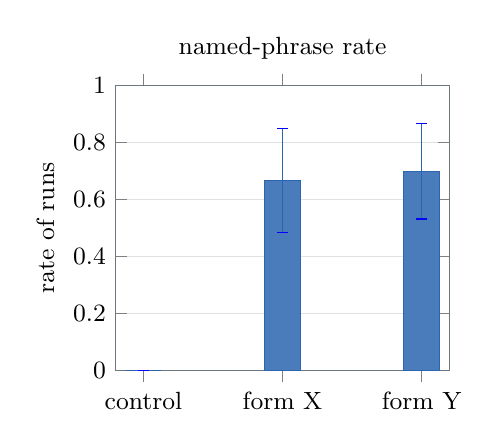
\begin{tikzpicture}
\begin{axis}[width=0.48\textwidth,height=5.2cm,ybar,bar width=13pt,
  ymin=0,ymax=1.0,ylabel={rate of runs},title={\small named-phrase rate},
  symbolic x coords={control,form X,form Y},xtick=data,
  axis line style={inkmut},tick label style={font=\small},
  ylabel style={font=\small},ymajorgrids,grid style={inkmut!22},
  error bars/y dir=both,error bars/y explicit]
\addplot+[fill=accent!85,draw=accent] coordinates {
  (control,0.000) +- (0,0)
  (form X,0.667) +- (0.207,0.182)
  (form Y,0.698) +- (0.174,0.167)};
\end{axis}
\end{tikzpicture}\hfill
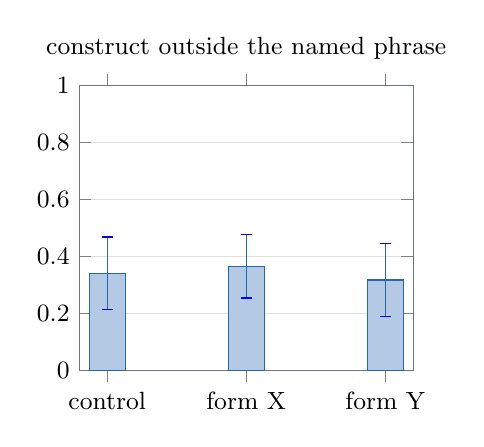
\begin{tikzpicture}
\begin{axis}[width=0.48\textwidth,height=5.2cm,ybar,bar width=13pt,
  ymin=0,ymax=1.0,title={\small construct outside the named phrase},
  symbolic x coords={control,form X,form Y},xtick=data,
  axis line style={inkmut},tick label style={font=\small},
  ymajorgrids,grid style={inkmut!22},
  error bars/y dir=both,error bars/y explicit]
\addplot+[fill=accent!35,draw=accent] coordinates {
  (control,0.341) +- (0.119,0.127)
  (form X,0.365) +- (0.111,0.111)
  (form Y,0.317) +- (0.119,0.127)};
\end{axis}
\end{tikzpicture}
\caption{The phrase-swap cell (378 runs, cluster-bootstrap 95\% CIs over 18
cases). \textbf{Left}: each instructed arm produces its own named phrase in
about two thirds of runs; control never produces either, and cross-form
leakage is $0/252$. \textbf{Right}: the validated-judge construct rate
\emph{outside} the named phrase is statistically indistinguishable across
all three arms. The instruction's entire measurable effect is the phrase it
names.}
\label{fig:swap}
\end{figure}


\textbf{Design.} Three arms, 18 cases, 7 repeats (378 runs). The control
arm is the minimal writer prompt. The two treated arms append a
byte-identical clause differing in exactly three words: \emph{``When you
state a number that is an estimate rather than an established fact,
label it using the phrase `modeled at' ''} (form X) or \emph{``\ldots
`taken to be' ''} (form Y). Form X is the historically dictated house
form (11 registry entries across 9 prompt symbols); form Y was chosen
the day before the run, appears zero times in 2M characters of archive,
and matches form X's spontaneous rate exactly ($0/249$ clean-provenance
runs for both). A harness gate refuses to run unless each arm contains
exactly its own form and no other registry phrase.

\textbf{Compliance is form-tracking and the house form has no
privilege.} Form X appears in $0.667$ of its arm's outputs (bootstrap CI
vs.\ control \ci{+0.468}{+0.857}); form Y in $0.698$
(\ci{+0.524}{+0.865}); cross-form leakage is $0/252$ --- no treated run
ever produced the other arm's form, and no control run produced either (Figure~\ref{fig:swap}, left).
A phrase drilled through months of system prompts and a
day-old synonym perform identically: whatever the instruction engages,
it is not a learned disposition toward the trained-on words.

\textbf{Nothing survives the swap.} With each arm's own named phrase
subtracted, the validated-judge construct rate is statistically
unchanged: form X $0.341 \to 0.365$ (\ci{-0.079}{+0.111}); form Y
$0.341 \to 0.317$ (\ci{-0.103}{+0.087}) --- opposite nominal directions,
both spanning zero (Figure~\ref{fig:swap}, right). Emission is flat across arms (43.7--46.6 sentences),
so the null is not bought with silence. The registered minimum
detectable effect is $+0.224$ at the realized cluster count; the result
licenses ``no form-independent effect $\ge 0.22$,'' not ``zero.''

The instruction's entire measurable effect is the phrase it names.

\section{The preference cell: the lift is real, and the phrase costs
preference}
\label{sec:pref}

\begin{figure}[t]
\centering
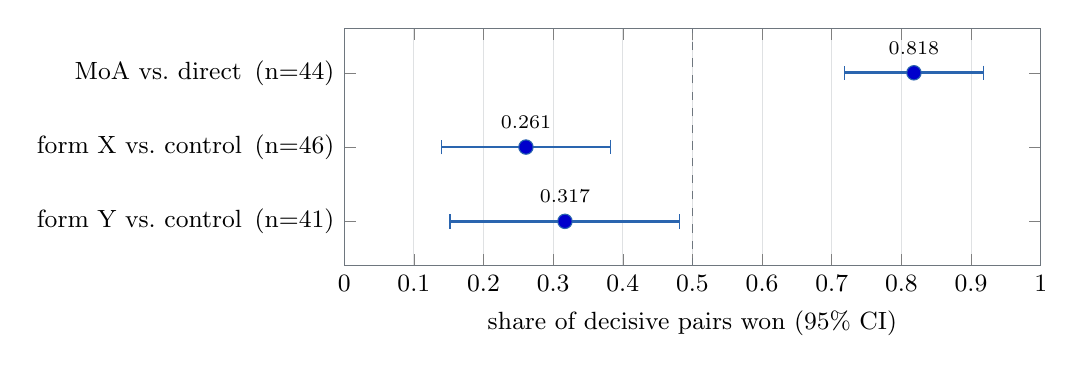
\begin{tikzpicture}
\begin{axis}[width=0.86\textwidth,height=4.6cm,xmin=0,xmax=1,
  ytick={1,2,3},yticklabels={form Y vs.\ control\, (n=41),
  form X vs.\ control\, (n=46), MoA vs.\ direct\, (n=44)},
  ymin=0.4,ymax=3.6,xlabel={share of decisive pairs won (95\% CI)},
  tick label style={font=\small},xlabel style={font=\small},
  axis line style={inkmut},xmajorgrids,grid style={inkmut!22}]
\addplot+[only marks,mark=*,mark size=2.6pt,color=accent,
  error bars/.cd,x dir=both,x explicit,error bar style={line width=1pt}]
  coordinates {
  (0.818,3) +- (0.100,0.101)
  (0.261,2) +- (0.121,0.127)
  (0.317,1) +- (0.165,0.163)};
\addplot[dashed,inkmut] coordinates {(0.5,0.4) (0.5,3.6)};
\node[font=\scriptsize,anchor=south] at (axis cs:0.818,3.12) {0.818};
\node[font=\scriptsize,anchor=south] at (axis cs:0.261,2.12) {0.261};
\node[font=\scriptsize,anchor=south] at (axis cs:0.317,1.12) {0.317};
\end{axis}
\end{tikzpicture}
\caption{The preference cell (order-debiased; a pair is decisive only when
the same side wins both orderings; cluster-bootstrap CIs over cases). The
aggregated pipeline beats the matched-length direct baseline decisively;
both phrase-instructed arms \emph{lose} to their own control, in
counterbalanced forms whose only difference from control is the phrase.
The dashed line is indifference.}
\label{fig:pref}
\end{figure}


\textbf{Design.} Three pairwise comparisons on the same 18 cases
(126 pairs each; both orderings; decisive only when the same side wins
both; primary judge \texttt{gpt-oss:20b}, which also wrote every output
on both sides of every pair, making self-preference symmetric by
construction). C1 pairs the phrase-swap control arm (the 2-layer MoA)
against a generated direct arm: the same writer, same cases, same
sampling, with the writer prompt minus only the sentence referencing
contributions. C2 and C3 pair each instructed arm against control ---
and because \S\ref{sec:phrase} established those arms differ only in
the phrase, any preference gap is causally the phrase's.

\textbf{The lift replicates at 20B scale.} The aggregated side wins
$0.818$ \ci{0.718}{0.919} of 44 decisive pairs. Arm mean lengths differ
by $1.4\%$ (7{,}757 vs.\ 7{,}649 chars), and the share among
near-length-matched pairs is $0.815$, so the lift is not length (Figure~\ref{fig:pref}). It also
does not track domain-framework density (the winner has more frameworks
per kilocharacter in only $0.409$ of decisive pairs). Its composition is
\emph{unidentified} by our feature set --- reported as such.

\textbf{The phrase arms lose, in both forms.} The instructed arms'
shares against their own control are $0.261$ \ci{0.140}{0.388} (form X)
and $0.317$ \ci{0.152}{0.480} (form Y): both confidence intervals lie
entirely below $0.5$, in the same direction, across counterbalanced
forms, and the penalty survives length matching. Our registered
prediction was the opposite (that judges reward the compliance
register); the result is a falsification-by-reversal, and is stronger
than the prediction: \textbf{dictated epistemic marking costs preference
points}.

\textbf{The tension, stated.} Chaining \S\ref{sec:phrase} and
\S\ref{sec:pref}, both links causal: an epistemic instruction installs
only a surface form; a preference judge penalizes that form. A pipeline
tuned toward judge preference --- RLHF-style or best-of-$n$ against a
preference model --- will therefore shed exactly the epistemic marking
that instruction paradigms install, while leaving the underlying
disposition (unchanged by the instruction anyway) untouched. Preference
optimization and epistemic disposition are not merely unaligned; at this
scale they are measurably opposed at the surface where instructions act.

\section{Mechanisms the MoA narrative assumes}
\label{sec:mech}

\begin{figure}[t]
\centering
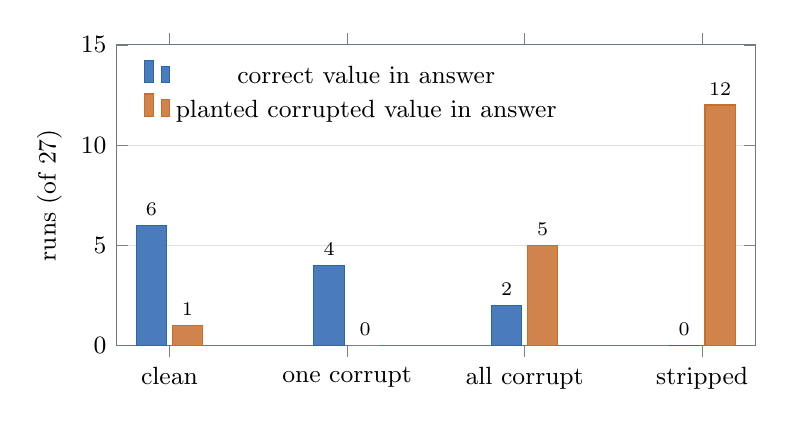
\begin{tikzpicture}
\begin{axis}[width=0.8\textwidth,height=5.4cm,ybar,bar width=11pt,
  ymin=0,ymax=15,ylabel={runs (of 27)},
  symbolic x coords={clean,one corrupt,all corrupt,stripped},xtick=data,
  axis line style={inkmut},tick label style={font=\small},
  ylabel style={font=\small},ymajorgrids,grid style={inkmut!22},
  legend style={font=\small,draw=none,at={(0.03,0.97)},anchor=north west},
  nodes near coords,nodes near coords style={font=\scriptsize,text=black}]
\addplot+[fill=accent!85,draw=accent] coordinates {
  (clean,6) (one corrupt,4) (all corrupt,2) (stripped,0)};
\addplot+[fill=corrupt!85,draw=corrupt] coordinates {
  (clean,1) (one corrupt,0) (all corrupt,5) (stripped,12)};
\legend{correct value in answer,planted corrupted value in answer}
\end{axis}
\end{tikzpicture}
\caption{The source-selector gradient (planted arithmetic errors; exact
match on known values). As clean sources are removed --- one proposer
corrupted, all corrupted, working stripped --- adoption of the planted
wrong value rises monotonically $1\to0\to5\to12$ while correct values
vanish. The aggregator prefers uncorrupted sources when they exist and has
no independent hold on the content when they do not.}
\label{fig:grad}
\end{figure}


\textbf{The aggregator selects sources; it does not recompute.} With
arithmetic claims planted in proposer texts: when one proposer is
corrupted and a clean one remains, the corrupted value reaches the
answer $0/27$ times; when every proposer is corrupted, $5/27$; when the
working is also stripped, $12/27$. The monotone gradient
$1\to0\to5\to12$ across arms (Figure~\ref{fig:grad}) identifies preference for uncorrupted
sources with no independent recomputation. MoA's own evidence that the
aggregator's output overlaps most with the best proposals
\cite{wang2024moa} is the same phenomenon viewed from the benign side;
the planted-error view adds its failure boundary, and shows the
``collaborativeness even from worse inputs'' claim fails at the fact
level: worse inputs made the writer factually worse.

\textbf{Corroboration is ignored.} Claims advanced by $k\ge2$
independent proposers transport to the final answer no more often than
single-proposer claims ($0.487$ vs.\ $0.524$; difference CI
\ci{-0.153}{+0.080}, excluding gains above $+0.08$) --- the one
reliability signal the architecture uniquely provides is unused.

\textbf{Transport is weak; invention is real.} On de-scaffolded arms
under the validated instrument, the writer transports upstream epistemic
qualification with slope $w = 0.150$ \ci{0.058}{0.252} (one writer;
second writer's CI includes zero at $n{=}20$), and invents qualification
at a $0.333$ \ci{0.138}{0.609} rate on inputs confirmed to contain none.

\textbf{Mixing is not automatically diverse.} Two medical fine-tunes of
the \emph{same} base model do not share a domain signature: one shifts
in-domain framework density $+0.232$ \ci{+0.072}{+0.412} over the base,
the other $+0.109$ \ci{-0.056}{+0.300}, and a second lineage shows
$-0.041$ \ci{-0.099}{+0.025} --- per-model, not per-domain-training.
A post-hoc descriptive check (not a registered result) further found two
same-domain seats no more distant from each other than one seat is from
itself across samples; registered or not, the published Self-MoA result
\cite{li2025selfmoa} independently reaches the same conclusion at
benchmark scale.

\textbf{Accuracy.} On a 60-item self-verifying battery the aggregated
pipeline and the bare writer are statistically indistinguishable, but
the comparison sits at a $0.92$--$0.97$ ceiling with three discordant
items; per our audit discipline this is held as absence of evidence, not
evidence of absence.

\section{Discussion}

\textbf{What the lift is, and is not.} The audit does not debunk MoA's
headline: aggregation genuinely wins preference at our scale, under a
debiased protocol, against a matched-length direct baseline. What it
removes is the assumed mechanism story. The lift is not built from the
epistemic behaviors the aggregate prompt requests (those requests
install phrases, and the judge penalizes them), not from length, and not
from domain-framework density; and the aggregator beneath it selects
rather than verifies. The residual --- plausibly organization,
coverage, or specificity harvested from proposers --- is the right
target for the next instrument, and we decline to name it without one.

\textbf{Implication for preference-trained pipelines.} The measured
tension predicts that preference optimization silently strips epistemic
marking. This is consistent with, and sharpens, verbosity- and
sycophancy-style results \cite{singhal2023length,sharma2023sycophancy}:
the pressure is not merely toward longer or more agreeable text but
away from the specific surface forms by which pipelines currently
signal uncertainty. Systems that must retain calibrated marking under
preference pressure will need it carried somewhere preference cannot
see --- structured fields, tool outputs --- rather than in-band prose.

\textbf{Implication for evaluation.} At auditable scale, five sixths of
a raw preference verdict is reading order. Single-ordering LLM-judge
evaluations at this scale are measuring position; debiased protocols
are usable but must budget for a ${\sim}0.35$ decisive rate.

\section{Limitations}

One preference judge (which is also the writer; symmetric but
family-specific), one aggregator family, 7--20B scale --- the tension
should be retested with larger judges and disjoint writer/judge
families. The case battery is advisory-domain and English-only. The
phrase-swap cell's null licenses only effects ${\ge}0.22$; the
preference cell's decisive $n$ (44) gives a minimum detectable share of
${\sim}0.67$, which the observed $0.818$ clears but subtler lifts would
not. Several early program values remain PROVISIONAL pending
re-measurement and are not used here. Claims marked single-judge or
single-writer should not be generalized past their scope.

\section{Reproducibility}

The measurement kit (\texttt{gst}: record contracts, pure-stdlib
statistics, instruments, registry and gates), the frozen dictation
registry and form-freeze files, all pre-registrations with their
falsification conditions and attainability computations, every deviation
and verdict, and the three program audits are in the project repository;
each cell's registration is committed before its first run, so temporal
ordering is verifiable from history.

\begin{thebibliography}{9}
\bibitem{wang2024moa} J.~Wang, J.~Wang, B.~Athiwaratkun, C.~Zhang,
J.~Zou. Mixture-of-Agents enhances large language model capabilities.
\emph{arXiv:2406.04692}, 2024.
\bibitem{li2025selfmoa} W.~Li et al. Rethinking Mixture-of-Agents: is
mixing different large language models beneficial?
\emph{arXiv:2502.00674}, 2025.
\bibitem{zheng2023judging} L.~Zheng et al. Judging LLM-as-a-judge with
MT-Bench and Chatbot Arena. \emph{NeurIPS Datasets and Benchmarks},
2023.
\bibitem{singhal2023length} P.~Singhal et al. A long way to go:
investigating length correlations in RLHF. \emph{arXiv:2310.03716},
2023.
\bibitem{sharma2023sycophancy} M.~Sharma et al. Towards understanding
sycophancy in language models. \emph{arXiv:2310.13548}, 2023.
\bibitem{wang2024rebuttal} Q.~Wang et al. Rethinking the bounds of LLM
reasoning: are multi-agent discussions the key? \emph{arXiv:2402.18272},
2024.
\end{thebibliography}

\end{document}
